%*----------- SLIDE -------------------------------------------------------------
\begin{frame}[c]{The Stanford Cart}
    \begin{columns}
        \column{.05\textwidth}
        \column{.45\textwidth}
        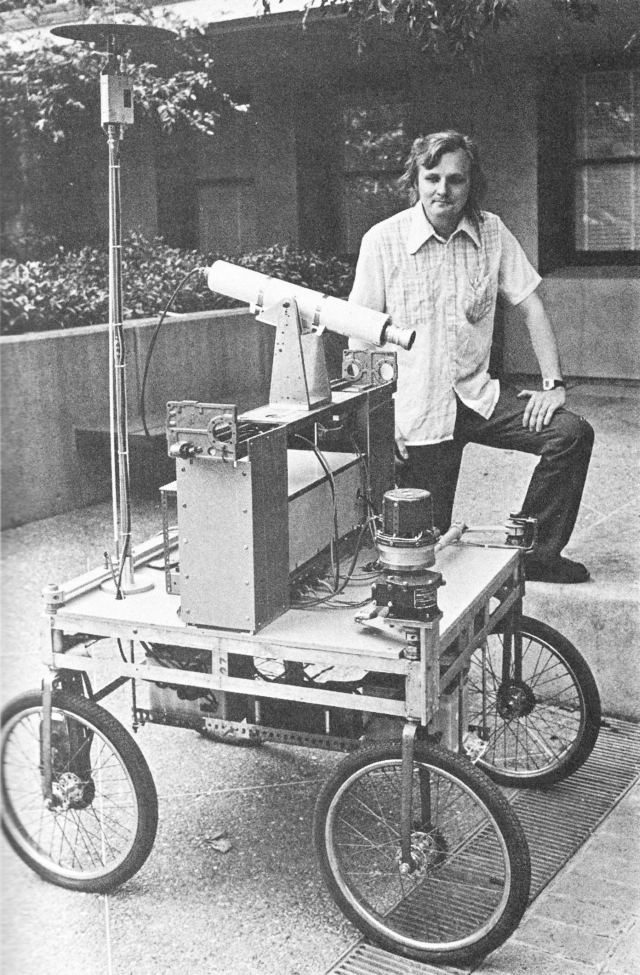
\includegraphics[width=0.6\textwidth, clip, trim = 0 0 0 0]{TheStanfordCart/StanfordCart-Moravec-x640.jpg}
        \column{.5\textwidth}
            % \centering
            TV-equipped mobile robot
            \begin{itemize} 
                \item Created by Hans. P. Moravec
                \item It was minimal remotely controlled
                \item Used stereo vision
            \end{itemize}
            \singlespacing
            Cart's systems
            \begin{itemize}
                \item Reliable for shorts runs, but slow
                \item There were some problems in its rotines
                 \end{itemize}
            % \includegraphics[width=0.8\textwidth, clip, trim = 0 0 0 0]{colab-logo.png}
    \end{columns}
%*----------- notes
    \note[item]{Notes can help you to remember important information. Turn on the notes option.}
\end{frame}
%-
%*----------- SLIDE -------------------------------------------------------------
\begin{frame}[t]{The Stanford Cart's Rotines}
    %\transboxout[duration=0.5]
    \vspace*{0.3cm}
    O robô obtêm 9 fotos através de sua câmera, e a partir destas é capaz de
    deduzir a transfromada da sua coordenada 3D e a posição 3D dos features das imagens.
    
    \vspace*{0.3cm}

    Para planejar a sua trajetória o robô projetava os obstáculos no chão como circulos à serem evitados
  
    \vspace*{0.8cm}
    \centering
    
\includegraphics[width=0.8\textwidth, clip, trim = 0 0 0 0]{TheStanfordCart/diagram.png}
%*----------- notes
    \note[item]{Notes can help you to remember important information. Turn on the notes option.}
\end{frame}
%-
%*----------- SLIDE -------------------------------------------------------------
\begin{frame}[c]{Prática 1 - Resolução questão no Google Colab}
    \begin{columns}
        \column{.01\textwidth}
        \column{.50\textwidth}
        Google Colab
        \begin{itemize} 
            \item Colab é um ambiente de desenvolvimento Python executado no 
            navegador usando o Google Cloud
        \end{itemize}
        \singlespacing
        Bibliotecas:
        \begin{itemize}
            \item SymPy: é uma biblioteca Python para matemática simbólica
            \item Math: é um módulo integrado que fornece uma série de métodos e constantes matemáticas
        \end{itemize}
        \column{.5\textwidth}
            \centering
            \includegraphics[width=0.8\textwidth, clip, trim = 0 0 0 0]{colab-logo.png}
    \end{columns}
%*----------- notes
    \note[item]{Notes can help you to remember important information. Turn on the notes option.}
\end{frame}
%-

%*----------- SLIDE -------------------------------------------------------------
\begin{frame}[c]{Tipos de juntas}
    %\transboxout[duration=0.5]
    \centering
    \includegraphics[width=0.8\textwidth, clip, trim = 0 0 0 0]{tipos-juntas.png}
%*----------- notes
    \note[item]{Notes can help you to remember important information. Turn on the notes option.}
\end{frame}
%-

%*----------- SLIDE ------------------------------------------------------------
\begin{frame}
    %\transdissolve[duration=0.5]
    %\hspace*{-1cm}
    \begin{columns}
        %\column{.01\textwidth}
        \column{0.50\textwidth}
        ~\hfill
            \begin{beamercolorbox}[sep=8em, colsep*=18pt, wd=\textwidth,ht=\paperheight]{title page header}
                \begin{center}
                    \textbf{\huge{GRAUS DE}}\par
                    \vspace*{0.3cm}
                    \textbf{\huge{LIBERDADE}}\par
                    \vspace*{0.3cm}
                    é definido como a maneira pela qual um robô ou máquina pode se mover.
                \end{center}
            \end{beamercolorbox}%         
        \column{.05\textwidth} 
        \column{.65\textwidth}
        \begin{center}
            \includegraphics[width=.8\textwidth]{gdl.png}
        \end{center}
            
    \end{columns}
  
%*----------- notes
    \note[item]{Notes can help you to remember important information. Turn on the notes option.}
 \end{frame}
%-